%%%%%%%%%%%%%%%%%%%%%%%%%%%%%%%%%%%%%%%%%%%%%%%%%%%%%%%%%%%%%%%%%%%%%%%%%%%%%%%%
%2345678901234567890123456789012345678901234567890123456789012345678901234567890
%        1         2         3         4         5         6         7         8

% \documentclass[letterpaper, 10 pt, conference]{ieeeconf}  % Comment this line 
% out if you need a4paper

\documentclass[usletter, 10pt, conference]{ieeeconf}      % Use this line for a4 
% paper
\usepackage{graphicx}\graphicspath{{figures/}}
\usepackage{todonotes}
\renewcommand{\todo}[1]{\textcolor{magenta}{[TODO: #1]}}
\usepackage{amsmath,amsfonts,euscript,amscd,amssymb}
% \numberwithin{equation}{chapter}
% \usepackage{caption}
% \captionsetup[figure]{figurewithin=chapter}
% \numberwithin{table}{chapter}
% \usepackage{multirow, setspace} 
% \usepackage{subfigure}
\usepackage{graphicx}
\usepackage{caption}
\usepackage{subcaption}
\usepackage{algorithm}
\usepackage{algorithmic} 
\usepackage{epsfig}
\usepackage{enumerate}
\usepackage{gensymb}
\usepackage{notoccite}
\usepackage{svg}
\usepackage{url}
\pdfminorversion=4
% \usepackage[noadjust]{cite}
% \usepackage{cite}
% \usepackage[utf8x]{inputenc}
% % functions
% \newcommand{\estimated}[1]{\hat{#1}}
% \newcommand{\qindent}{\hspace{4em}}
% 
% % general


\newcommand{\R}{\mathbb{R}}
% rigid body dynamics
\newcommand{\qdot}{\dot{q}}             % joint velocity
\newcommand{\qddot}{\ddot{q}}           % joint acceleration
\newcommand{\bq}{\mathbf{q}}            % (bold) joint position
\newcommand{\bqdot}{\dot{\bq}}          % (bold) joint velocity
\newcommand{\bqddot}{\ddot{\bq}}        % (bold) joint acceleration
\newcommand{\bM}{\mathbf{M}}            % inertia matrix
\newcommand{\bMt}{\tilde{\mathbf{M}}} 
\newcommand{\bh}{\mathbf{h}}    
\newcommand{\bS}{\mathbf{S}}    
\newcommand{\VF}{\mathbf{V}}  
\newcommand{\bR}{\mathbf{R}}  
\newcommand{\bQ}{\mathbf{Q}}  
\newcommand{\bJ}{\mathbf{J}} 
\newcommand{\bzero}{\mathbf{0}} 
\newcommand{\bP}{\mathbf{P}}  
\newcommand{\traj}{\mathbf{\tau}}
\newcommand{\bPsi}{\mathbf{\Psi}} 

\newcommand{\Cn}{\mathcal{C}}

 \newcommand{\bC}{\mathbf{C}} 
\newcommand{\bg}{\mathbf{g}} 
\newcommand{\bG}{\mathbf{G}} 
\newcommand{\bw}{\mathbf{w}} 
\newcommand{\Bfc}{\mathbf{f_c}} 
\newcommand{\bz}{\mathbf{z}}

\newcommand{\bV}{\mathbf{V}}    
\newcommand{\bD}{\mathbf{D}}     

\newcommand{\bI}{\mathbf{I}}   
\newcommand{\bv}{\mathbf{v}}            % velocities at contact
\newcommand{\blambda}{\mathbf{Y}} % forces at contact
\newcommand{\bK}{\mathbf{K}}            % Jacobian of mapping from generalised to contact 
\newcommand{\bKt}{\tilde{\mathbf{K}}}            % Jacobian of mapping from generalised to contact 
\newcommand{\bc}{\mathbf{c}}   		% compacting term (known terms)
\newcommand{\bff}{\mathbf{f}}   		% compacting term (contact impulse)
\newcommand{\bct}{\tilde{\mathbf{c}}}   		% compacting term (known terms)
\newcommand{\bA}{\mathbf{A}}     
\newcommand{\ba}{\mathbf{a}}     
\newcommand{\bF}{\mathbf{F}}     
\newcommand{\bB}{\mathbf{B}}    

\newcommand{\bl}{\mathbf{l}}  
\newcommand{\bL}{\mathbf{L}}  
\newcommand{\bLbar}{\bar {\mathbf{L}} }

\newcommand{\btau}{\boldsymbol{\tau}}   % (bold) torque

%optimal control
\newcommand{\dimU}{m} %dimensionality of control
\newcommand{\f}{\mathcal{F}} %dynamics function
\newcommand{\F}{\mathbf{F}} %dynamics function
\newcommand{\bu}{\mathbf{u}}  %control vector
\newcommand{\bx}{\mathbf{x}}  %state
\newcommand{\bp}{\mathbf{p}}  %state
\newcommand{\bs}{\mathbf{s}}  %state
% \newcommand{\bS}{\mathbf{S}}  %state
\newcommand{\tc}{\rho} %terminal cost
\newcommand{\rc}{r} %running cost
\newcommand{\J}{\mathbf{J}} %cost function
\newcommand{\dimX}{n}
\newcommand{\bxdot}{\dot{\bx}}          % state time derivative
\newcommand{\g}{\mathcal{G}} %stochasticity in dynamics

\newcommand{ \probability}{\mathsf{p}}            % 
\newcommand{\lambdaLM}{\beta}            % LM scalar iLQG

\newcommand{\tp}{\mathit{tp}}
\newcommand{\z}{\mathit{z}}
\newcommand{\bxp}{\bx'}  
\newcommand{\scost}{\mathit{o}} % state cost function

\newcommand{\mbf}{\mathbf}

\newcommand{\gMAT}{\mathbf{G}}

\newcommand{\bbx}   {\bar{\bx}}         % nominal state sequence
\newcommand{\bbu}   {\bar{\bu}}         % nominal command sequence

\newcommand{\fx}   {\f_\bx}             % dynamics function derivative w.r.t. x
\newcommand{\fu}   {\f_\bu}             % dynamics function derivative w.r.t. u
\newcommand{\hx}   {\tc_\bx}              % terminal cost function derivative w.r.t. x
\newcommand{\hxx}  {\tc_{\bx\bx}}         % terminal cost function 2nd derivative w.r.t. x
\newcommand{\lx}   {\rc_\bx}              % running cost function derivative w.r.t. x
\newcommand{\lu}   {\rc_\bu}              % running cost function derivative w.r.t. u
\newcommand{\lxx}  {\rc_{\bx\bx}}         % running cost function 2nd derivative w.r.t. x
\newcommand{\luu}  {\rc_{\bu\bu}}         % running cost function 2nd derivative w.r.t. u
\newcommand{\lxu}  {\rc_{\bx\bu}}         % running cost function cross derivative

\newcommand{\xbar}{\bar{\mathbf{x}}}
\newcommand{\ubar}{\bar{\mathbf{u}}}
\newcommand{\Jbar}{\bar{\J}}

\newcommand{\Jxx}  {\J_{\bx\bx}}         % running cost function 2nd derivative w.r.t. x
\newcommand{\Juu}  {\J_{\bu\bu}}         % running cost function 2nd derivative w.r.t. u
\newcommand{\Jxu}  {\J_{\bx\bu}} 

\newcommand{\utilde}{\tilde{\mathbf{u}}}
\newcommand{\xtilde}{\tilde{\mathbf{x}}}
\newcommand{\Jtilde}{\tilde{\J}}
\newcommand{\Hfix}{\mathcal{H}}
\newcommand{\Ham}{\mathbf{H}}


\newcommand{\dt}{\mathrm{d}t}


\def \BDelta { {\bf \Delta} }
\def \Real { \mathbb{R} }

 \newcommand{\dimQ}{\dimX}
\newcommand{\dimC}{\dimU}
%%%%%%%%%%% useful math stuff %%%%%%%%%%%
\newcommand{\twovec}[2]{\left[\begin{array}{c}
                                  #1\\ #2\\
                            \end{array}
                       \right]}
\newcommand{\threevec}[3]{\left[\begin{array}{c}
                                  #1\\ #2\\ #3 \\
                            \end{array}
                       \right]}
\newcommand{\fourvec}[4]{\left[\begin{array}{c}
                                  #1\\ #2\\ #3 \\ #4\\
                            \end{array}
                       \right]}

\newcommand{\tworvec}[2]{\left[\begin{array}{cc}
                                  #1 & #2\\
                            \end{array}
                       \right]}

\newcommand{\threervec}[3]{\left[\begin{array}{ccc}
                                  #1 & #2 & #3\\
                            \end{array}
                       \right]}

\newcommand{\fourrvec}[4]{\left[\begin{array}{cccc}
                                  #1 & #2 & #3 & #4\\
                            \end{array}
                       \right]}

\newcommand{\twovect}[2]{[\;#1,\;#2\;]^T}
\newcommand{\threevect}[3]{[\;#1,\;#2,\;#3\;]^T}
\newcommand{\fourvect}[4]{[\;#1,\;#2,\;#3,\;#4\;]^T}
\newcommand{\twomatrix}[4]{ \left[\begin{array}{cc}
                                   #1 & #2\\
                                   #3 & #4\\
                                 \end{array}
                           \right]}
\newcommand{\threematrix}[9]{ \left[\begin{array}{ccc}
                                   #1 & #2 & #3 \\
                                   #4 & #5 & #6 \\
				   #7 & #8 & #9 \\
                                 \end{array}
                           \right]}
\newcommand{\eqdef}{\stackrel{\rm def}{=}}
\newcommand{\diag}{\mathrm{diag}}

% partial derivatives
\newcommand{\partiald}[2]{
\frac{\partial #1}{\partial #2}}

\newcommand{\partialtwod}[2]{
\frac{\partial^{2} #1}{\partial #2}}

%%% definition of boldmath letters %%%

   %%% lower case Greek letters
\def \Balpha      { {\mbox{\boldmath $\alpha$}}}
\def \Bbeta       { {\mbox{\boldmath $\beta$}}}
\def \Bgamma      { {\mbox{\boldmath $\gamma$}}}
\def \Bdelta      { {\mbox{\boldmath $\delta$}}}
\def \Bepsilon    { {\mbox{\boldmath $\epsilon$}}}
\def \Bvarepsilon { {\mbox{\boldmath $\varepsilon$}}}

\def \Bzeta       { {\mbox{\boldmath $\zeta$}}}
\def \Beta        { {\mbox{\boldmath $\eta$}}}
\def \Btheta      { {\mbox{\boldmath $\theta$}}}
\def \Bvartheta   { {\mbox{\boldmath $\vartheta$}}}
\def \Biota       { {\mbox{\boldmath $\iota$}}}

\def \Bkappa      { {\mbox{\boldmath $\kappa$}}}
\def \Blambda     { {\mbox{\boldmath $\lambda$}}}
\def \Bmu         { {\mbox{\boldmath $\mu$}}}
\def \Bnu         { {\mbox{\boldmath $\nu$}}}
\def \Bxi         { {\mbox{\boldmath $\xi$}}}
\def \Bomicron    { {\mbox{\boldmath $o$}}}

\def \Bpi         { {\mbox{\boldmath $\pi$}}}
\def \Bphi        { {\mbox{\boldmath $\phi$}}}
\def \Brho        { {\mbox{\boldmath $\rho$}}}
\def \Bvarrho     { {\mbox{\boldmath $\varrho$}}}
\def \Bsigma      { {\mbox{\boldmath $\sigma$}}}
\def \Bvarsigma   { {\mbox{\boldmath $\varsigma$}}}

\def \Btau        { {\mbox{\boldmath $\tau$}}}
\def \Bupsilon    { {\mbox{\boldmath $\upsilon$}}}
\def \Bphi        { {\mbox{\boldmath $\phi$}}}
\def \Bvarphi     { {\mbox{\boldmath $\varphi$}}}
\def \Bchi        { {\mbox{\boldmath $\chi$}}}
\def \Bpsi        { {\mbox{\boldmath $\psi$}}}
\def \Bomega      { {\mbox{\boldmath $\omega$}}}


   %%% upper case Greek letters
\def \BAlpha      { {\bf A} }
\def \BBeta       { {\bf B} }
\def \BGamma      { {\bf \Gamma} }
\def \BDelta      { {\bf \Delta} }
\def \BEpsilon    { {\bf E} }

\def \BZeta       { {\bf Z} }
\def \BEta        { {\bf H} }
\def \BTheta      { {\bf \Theta} }
\def \BIota       { {\bf I} }

\def \BKappa      { {\bf K} }
\def \BLambda     { {\bf \Lambda} }
\def \BMu         { {\bf M} }
\def \BNu         { {\bf N} }
\def \BXi         { {\bf \Xi} }
\def \BOmicron    { {\bf O} }

\def \BPi         { {\bf \Pi} }
\def \BPhi        { {\bf \Phi} }
\def \BRho        { {\bf P} }
\def \BSigma      { {\bf \Sigma} }

\def \BTau        { {\bf T} }
\def \BUpsilon    { {\bf \Upsilon} }
\def \BPhi        { {\bf \Phi} }
\def \BChi        { {\bf X} }
\def \BPsi        { {\bf \Psi} }
\def \BOmega      { {\bf \Omega} }

   %%% lower case bold letters
\def \Ba { {\bf a} }
\def \Bb { {\bf b} }
\def \Bc { {\bf c} }
\def \Bd { {\bf d} }
\def \Be { {\bf e} }
\def \Bf { {\bf f} }
\def \Bg { {\bf g} }
\def \Bh { {\bf h} }
\def \Bi { {\bf i} }
\def \Bj { {\bf j} }
\def \Bk { {\bf k} }
\def \Bl { {\bf l} }
\def \Bm { {\bf m} }
\def \Bn { {\bf n} }
\def \Bo { {\bf o} }
\def \Bp { {\bf p} }
\def \Bq { {\bf q} }
\def \Br { {\bf r} }
\def \Bs { {\bf s} }
\def \Bt { {\bf t} }
\def \Bu { {\bf u} }
\def \Bv { {\bf v} }
\def \Bw { {\bf w} }
\def \Bx { {\bf x} }
\def \By { {\bf y} }
\def \Bz { {\bf z} }

   %%% upper case bold letters
\def \BA { {\bf A} }
\def \BB { {\bf B} }
\def \BC { {\bf C} }
\def \BD { {\bf D} }
\def \BE { {\bf E} }
\def \BF { {\bf F} }
\def \BG { {\bf G} }
\def \BH { {\bf H} }
\def \BI { {\bf I} }
\def \BJ { {\bf J} }
\def \BK { {\bf K} }
\def \BL { {\bf L} }
\def \BM { {\bf M} }
\def \BN { {\bf N} }
\def \BO { {\bf O} }
\def \BP { {\bf P} }
\def \BQ { {\bf Q} }
\def \BR { {\bf R} }
\def \BS { {\bf S} }
\def \BT { {\bf T} }
\def \BU { {\bf U} }
\def \BV { {\bf V} }
\def \BW { {\bf W} }
\def \BX { {\bf X} }
\def \BY { {\bf Y} }
\def \BZ { {\bf Z} }

%%%  bold numbers
\def \Bzero { {\bf 0} }
\def \Bone  { {\bf 1} }

%%% Re %%% need \usepackage{amsfonts}
\usepackage{amsfonts}
\def \Real { \mathbb{R} }

\newtheorem{theorem}{Theorem}
\newtheorem{lemma}{Lemma}
\newtheorem{definition}{Definition}

%%% end of math stuff


\IEEEoverridecommandlockouts                              % This command is only 
% needed if 
                                                          % you want to use the 
% \thanks %command

\overrideIEEEmargins                                      % Needed to meet 
% printer requirements.

% See the \addtolength command later in the file to balance the column lengths
% on the last page of the document

% The following packages can be found on http:\\www.ctan.org
%\usepackage{graphics} % for pdf, bitmapped graphics files
%\usepackage{epsfig} % for postscript graphics files
%\usepackage{mathptmx} % assumes new font selection scheme installed
%\usepackage{times} % assumes new font selection scheme installed
%\usepackage{amsmath} % assumes amsmath package installed
%\usepackage{amssymb}  % assumes amsmath package installed

\title{\LARGE \bf Whole-body Trajectory Optimization for \\ Non-periodic Dynamic 
Motions on Quadrupedal Systems}

\author{Andreea Radulescu$^{1}$  Ioannis Havoutis$^{2,3}$ Darwin G. Caldwell$^1$ Claudio Semini$^{1}$ 
\thanks{*This research is funded by the Fondazione Istituto Italiano di Tecnologia}% <-this % stops a space
\thanks{$^{1}$Department of Advanced Robotics, Istituto Italiano di
Tecnologia, via Morego, 30, 16163 Genova, Italy. \textit{email}: 
% {andreea.radulescu, claudio.semini}@iit.it}
        {\tt\small \{andreea.radulescu, darwin.caldwell,  claudio.semini\}@iit.it}}%
\thanks{$^{2}$Robot Learning and Interaction Group, Idiap Research Institute, 
Martigny, Switzerland \textit{email}: {\tt\small ioannis.havoutis@idiap.ch}}%
\thanks{$^{3}$Oxford Robotics Institute, Department of Engineering Science, University of Oxford, United Kingdom. {\tt\small ihavoutis@robots.ox.ac.uk}}%
}

% video link
% https://youtu.be/irZTaTgwdoE

% https://youtu.be/irZTaTgwdoE

\begin{document}

\maketitle
\thispagestyle{empty}
\pagestyle{empty}

%%%%%%%%%%%%%%%%%%%%%%%%%%%%%%%%%%%%%%%%%%%%%%%%%%%%%%%%%%%%%%%%%%%%%%%%%%%%%%%%
\begin{abstract}
Autonomous legged robots will be required to handle a wide range of tasks 
in complex environments. While a lot of research has focused on developing 
their abilities for periodic locomotion tasks, less effort has been invested 
in devising generalized strategies for dynamic, 
non-periodic movements. Motion design approaches are frequently enlisted in the form of 
teleoperation or predefined heuristics in such scenarios. We employ a realistic 
simulation of the hydraulically actuated HyQ2Max quadrupedal system for 
investigations on two distinctive tasks: rearing and posture recovery. 
We present a whole-body optimization methodology for non-periodic tasks on quadrupedal systems. 
This approach delivers solutions involving multiple contacts without 
the need for predefined feet placements. 
The results obtained show the potential of optimization approaches for 
motion synthesis in the context of complex tasks.
\end{abstract}

\begin{keywords}
\textit{optimization, parametrized policy, multi-legged systems, switching contacts,
non-periodic movements, quadruped, posture recovery, whole-body trajectory}
\end{keywords}

\section{Introduction}

Modern robotic systems come in diverse configurations depending on their function. 
As a consequence of the wide range of applications, complex designs emerged to meet their demands.
Controlling such complex robotic systems is a challenging task, 
due to the kinematic and actuation redundancies and due to discontinuities in the 
dynamics, introduced by switching contact conditions with the environment. 

Biological legged systems can achieve a variety of whole body movements, in order to manipulate
and traverse their environment. They exercise control over their limbs with significant versatility, compliance and energy 
efficiency. This performance is achieved despite noticeable levels of delay and noise affecting the biological 
motor systems \cite{faisal2008noise}. When transferring these skills to their robotic counterparts,
most research has focused on periodic tasks, frequently designed with respect to a stability criterion, such as trotting and walking. 

A fully autonomous locomotion system will have to complete a heterogeneous range of tasks.
Some of these frequent tasks in complex environments will require non-periodic solutions which can be described as single-shot movements.
Examples in quadrupedal locomotion include rearing, overcoming an obstacle or gap, 
squat-jumping in place, posture and fall recovery. 

Currently, the majority of robotic systems operating in an unsafe, disorganized and cluttered 
environment (e.g., search and rescue missions, disaster response, nuclear decommissioning) have to rely 
heavily on teleoperation in order to achieve their objectives. Extending the autonomy level of 
legged systems with such dynamic capabilities would ease the workload of the human operators. 
Taking into consideration the time-sensitive nature of some of these tasks, the presence of a large motion library would 
facilitate the improvement of the overall performance of the system.

Optimization and learning methodologies could deliver solutions for such scenarios 
by using high-level task specifications, in the form of an evaluation criterion 
of the overall performance of the emerging behavior. 

In this work we present a whole-body optimization methodology for non-periodic tasks on quadrupedal systems.
We encode the high-level goals using a task specific cost function, which provides an intuitive way of 
defining the desired outcome. Although tuning the relative weights of such cost functions is a manual 
process, a heuristic encoding of the same behavior would require a significantly higher effort.
The resultant trajectories and their performance indicate the capability of the approach to
deliver diverse sets of motions, without prior definitions for the feet placements.

\section{State of the art}

The relationship between learning and optimization has been under analysis for a long time
\cite{bennett2006interplay,kober2013reinforcement}. However, it is only in the recent past
that their use has been extended to high dimensional problems, common to modern
multi-degree-of-freedom robotics applications. The use of policy based formulations, 
rather than value function based ones, allows the integration of task/domain specific knowledge 
in the pre-structure of the policy. This allows the optimization methods to 
focus the search in promising areas of the space.

Various optimization approaches were proposed for dealing with multiple contact events. 
In \cite{Erez2011}, on-line Model Predictive Control (MPC) is combined with offline trajectory optimization. The 
limit cycle of a periodic movement is found by offline optimization with an infinite-horizon 
average cost, while on-line MPC is used to obtain an optimal feedback control law. Another study 
\cite{kulchenko2011}, generalizes MPC from the usual finite horizon (or receding horizon) setup to a 
first-exit setting (i.e., a solution is found based on the assumption of an exit state), which 
avoids dealing with discontinuities in the on-line optimization phase. 

The work in \cite{tassa_todorov.iros2012} proposes a locally optimal solution based on MPC with smooth
approximation of contact forces without the need of switching dynamics. In \cite{posa_tedrake.IJRR2014}, the contact 
forces are explicitly included as constraints (using complementarity conditions) and directly 
optimized, together with the trajectories and control commands, using sequential quadratic 
programming. 

Approaches such as Policy Improvement with Path Integrals ($PI^2$) \cite{theodorou2010generalized}, 
based on stochastic optimal control principles, have been successful in  generating 
optimal manipulation solutions for compliant robotic arms \cite{kalakrishnan2011learning}. In \cite{fankhauser2013reinforcement},
$PI^2$ is used on a combination of simulation and hardware based optimizations, to synthesize a periodic hopping behavior
for a one-legged system, in a number of scenarios. Using iterative optimal control, \cite{neunert2016trajectory} 
delivers locally optimal solutions for both periodic and non-periodic tasks on a quadrupedal system.

The Covariance Matrix Adaptation (CMA) algorithm \cite{hansen2001completely} 
has been similarly used to generate whole body movements. 
The study in \cite{shafii2015learning} employs the CMA Evolution Strategy 
(CMA-ES) to obtain an optimal fast walking solution
for both forward and sideways stepping. 
A preliminary study on the potential of CMA-ES was presented in \cite{havoutis2014optimization}, where the algorithm 
was used to obtain a rearing solution for the HyQ quadrupedal robotic system. 
In \cite{radulescu2016optimization} we conduct a preliminary study for the 
HyQ2Max platform for similar tasks. Likewise, in \cite{gehring2016practice}
the method is employed to achieve a squat-jump movement, as well as various periodic gaits.
The CMA method was shown to provide improved performance,
when compared with state-of-the-art global search methods \cite{hansen2004evaluating}, 
thus making it a method of choice for such investigations. 

Another major challenge is solving such high-level tasks without the use of 
pre-defined heuristics such as hard-coded sequences or feet 
placements \cite{Winkler2015}. Trajectory optimization for multi-legged robotic systems 
that operate in complex environments is challenging, due to the varying number 
of contacts. By allowing predefined elements, part of the burden is alleviated, 
but at the same time the solutions obtained might be suboptimal and their 
generality can also be affected. Recently, the work in \cite{clever2016novel} has combined optimal control and 
learning of movement primitives to generate gaits for a humanoid system, but the work is restricted to
open-loop control. 

In spite of the significant efforts in the area of fall avoidance, comparatively little research has focused
on developing generalized self-righting techniques. Most work has revolved around devising specific 
solutions for particular systems, either at hardware design level 
(low center of mass, invertible robots \cite{ben2008design}) or defining  embodiment specific strategies 
\cite{saranli2004model}. The work in \cite{kessens2014metric} is attempting to 
develop a generalized method for self-righting strategies, by analyzing and 
exploiting the given robot structure. However, the results are still restricted to 
small dimensional designs and do not address multi-legged systems (the study focuses on a tracked one-arm manipulator).

\section{Our methodology}

In our work we try to address this issue by providing a generalized approach of 
delivering whole body movement solutions. The high-level tasks are encoded 
using a cost function, while trying to avoid pre-specifying how these tasks 
should be solved (i.e., no predefined contact points or sequences). As the 
accuracy of the model is a crucial requirement, we choose to perform the optimization
using the whole body dynamics. 

\subsection{Robot description and System model}

We use a realistic simulation of the 80 kg HyQ2Max \cite{semini16tmech} 
quadrupedal robotic system with contacts. The platform was designed as a 
light-weight, robust locomotion vehicle and features 12 hydraulically actuated 
joints (controlled by a hydraulic valve). Each limb has 3 actuators, defined 
as: HAA (hip abduction/adduction), HFE (hip flexion/extension) and KFE (knee 
flexion/extension). The corresponding kinematic ranges are $90^{\circ}$, 
$270^{\circ}$, $165^{\circ}$, respectively. 

We model the behavior of the platform as a rigid body system defined as:
\begin{equation}
\bM \left( \bq \right) \ddot{\bq} + \bC \left( \bq, \dot{\bq} \right) \dot{\bq}+ 
\bg \left( \bq \right) + \bD \dot{\bq} = \bJ^T_{c} \lambda \left( \bq, 
\dot{\bq} \right) + \bS^{T} \btau,
\label{eq_motion_general}
\end{equation}
\noindent 
where $\bq = \left[\bq_{B}, \bx_{B}, \bq_{J} \right]^{T} $ is the vector containing 
the 6 DoF base state (orientation $\bq_{B}$, position $\bx_{B}$ of the trunk's Center of Mass (COM)) and the 
joint angles $\bq_{J}$,  with $\dot{\bq}, \ddot{\bq}$ the corresponding 
velocities and accelerations. The remaining notations are defined as following:
$ \bM $ is a symmetric positive definite inertia mass 
matrix, $ \bC$ represents centrifugal and Coriolis forces, $ \bg$ are the 
gravitational forces, $\bD$ is the viscous damping matrix. The contact forces 
$\lambda$ exert their effect on the system via the Jacobian $\J_{c}$, while the 
joint torques from the actuators $ \btau $ are mapped via the selection matrix 
$\bS$ onto the states.

The state vector of the HyQ2Max system is defined as:
\begin{equation}
 \bx = \left[  \bq ,   \dot{\bq} \right] ^{T} =
 \left[ \bq_{B}, \bx_{B}, \bq_{J}, \dot{\bq_{B}}, 
\dot{\bx_{B}}, \dot{\bq_{J}} \right] ^{T}
 \label{eq_state}
\end{equation}
\noindent 
where $ \bq , \dot{\bq}$ are the vectors defined 
for (\ref{eq_motion_general}), expressed in the world frame. The definitions of the
axes of the robot base frame are depicted in Fig. \ref{fig:rearing_behaviour} (left).

% The state vector of the HyQ2Max system is defined as:
% \begin{equation}
%  \bx = \left[ \omega \bq , \omega  \dot{\bq} \right] ^{T} =
%  \left[ \omega\bq_{B}, \omega\bx_{B}, \omega\bq_{J}, \omega\dot{\bq_{B}}, 
% \omega\dot{\bx_{B}}, \omega\dot{\bq_{J}} \right] ^{T}
%  \label{eq_state}
% \end{equation}
% \noindent 
% where $\omega \bq , \omega  \dot{\bq}$ are the $\bq, \dot{\bq}$ vectors defined 
% for Eq. \ref{eq_motion_general}, expressed in the global world frame $\omega$. 

The choice of contact model is crucial for ensuring the validity of the 
resultant trajectory. When considering the choice of models, there is always a
trade-off between numerical stability (smooth contact dynamics) and physical 
accuracy. 

% We use an ODE (Open Dynamics Engine) \cite{smith2002open} based contact model, where any 
% potential penetration errors are corrected at each time step (some penetration 
% threshold is tolerated in order to remove jitter) which provides a good gradient 
% of the dynamics. 

In the Open Dynamics Engine (ODE) \cite{smith2002open} contact model, any 
potential penetration errors are corrected at each time step (some penetration 
threshold is tolerated in order to remove jitter) which provides a good gradient 
of the dynamics. We employ Gazebo for our experiments, 
a well established simulation environment for robotic applications, which combines all the
functionalities of ODE with an increased user accessibility \cite{koenig2004design}.

\subsection{Optimization}

In our investigation we use a CMA-ES based approach to address dynamic 
non-periodic tasks for a quadrupedal robotic system: rearing and posture 
recovery. This technique proved effective in handling nonlinear, high-dimensional 
problems. The method operates by generating and evaluating 
a set of solutions at each iteration. The samples are extracted from a 
multivariate Gaussian distribution. After their evaluation 
the covariance matrix of the search distribution is adapted. 
% As this is a local 
% minimizer, an initial guess for the solution is provided at the start. 

For complex robotic systems such as HyQ2Max, the main challenge consists of 
determining the suitable joint motions which achieve the desired movement for 
each given task. Using a direct optimization approach on the time-parametrized joint or torque trajectories would involve an inconveniently large search 
space. Hence, we use a parametrized policy to encode these profiles, represented as 
a weighted average of Gaussian kernels: 
% \begin{eqnarray}
%  \label{weighted_sum}
%  f(t) & = & \sum_{i=1}^{M} w_i \phi_i(t)/ \sum_{i=1}^{M} \phi_i(t), \\
%  \phi_i(t) & = & exp(- \frac{1}{2 \sigma^2} (t-\mu_i)),
% \label{gaus_kernels}
% \end{eqnarray}
\begin{equation}
 \label{weighted_sum}
 f(t) = \sum_{i=1}^{M} w_i \phi_i(t)/ \sum_{i=1}^{M} \phi_i(t),
 \end{equation}
\noindent
where $w_i$ are the weights associated with each kernel $\phi_i, \; i \in [1, M]$, defined by mean $\mu_i$ and 
variance $\sigma^2$ as in:
\begin{equation}
 \phi_i(t) = exp(- \frac{1}{2 \sigma^2} (t-\mu_i)).
 \label{gaus_kernels}
\end{equation}

The CMA algorithm is then used to optimize the weights of all 
policies according to a task specific cost function (\ref{eq:cost_general}), applied to the 
whole body trajectory generated through (\ref{weighted_sum}) : 
\begin{equation}
 \label{eq:cost_general}
  J = p (\mathbf{s}_T, \mathbf{\dot{s}}_T)+\int^{T}_{t=0}\rc(\mathbf{\tau}_t, \bq_{J})\;\dt, \; t \in [0,T],
\end{equation}
\noindent
where $\mathbf{s}_t = [\bq_{B}, \bx_{B}]'$ is the trunk state (i.e., $\mathbf{s} 
= [x_{COM}, \; y_{COM}, \; z_{COM}, \; roll, \; pitch, \; yaw]'$)
% \begin{equation}
%  \mathbf{s} = [x_{COM}, \; y_{COM}, \; z_{COM}, \; roll, \; pitch, \; yaw]' 
% \label{eq:state_def}
% \end{equation}
% \noindent
and $\btau_t$ is the set of 12 torque actuation commands at time $t \in 
[0,T]$.

The cost function consists of a running term $ \rc $ that seeks 
to minimize the effort used for producing the motion and a final 
cost $p$ that evaluates the success of the motion according to the task goals 
(desired final states ($\bq^{*}_{B}, \bx^{*}_{B}$)) :
\begin{eqnarray}
 \label{eq:final_cost}
  \rc( \mathbf{s}_t, \mathbf{\dot{s}}_t, \mathbf{\tau}_t)  & = & Q_{3}  {\mathbf{\tau}_t}^{2} 
    + Q_{6} [(\bq_{J} - {\bq_{J}}_{max}))^2 \Big|_{\bq_{J}  > {\bq_{J}}_{max}} \\ \nonumber
    & + & (\bq_{J} - {\bq_{J}}_{min}))^2 \Big|_{\bq_{J}  < {\bq_{J}}_{min}}] \\ \nonumber
  p (\mathbf{s}_T, \mathbf{\dot{s}}_T) & = & (\bq_{B}(T) - \bq^{*}_{B})' Q_{1} (\bq_{B}(T) - \bq^{*}_{B}) \\ 
  & + & (\bx_{B}(T) - \bx^{*}_{B})' Q_{2} (\bx_{B}(T) - \bx^{*}_{B})
\end{eqnarray}
\noindent
where ${\bq_{J}}_{min},\; {\bq_{J}}_{max}$ are the upper and lower bounds on the joint limits $\bq_{J}$,
and $Q_{i}, \; i \in \{1,2,3,4\}$ are the relative weights associated with the terms for each individual task.


Since the CMA-ES is a local method, a starting policy is required.
In our experiments the policies are initialized with values that maintain an 
initial pose (in the case of rearing tasks) or as a direct interpolation 
between the initial configuration and desired final pose (for posture recovery).
No specific footstep sequence information is enforced. We apply 
a staged optimization approach, where preliminary solutions are obtained using 
a relaxed cost (e.g., lower weights for the joint limits term). The complexity of the cost 
function is increased gradually, until the solution meets all the desired 
requirements\footnote{We note that the robot model used incorporates a model of the
actuator dynamics, thus increasing the feasibility of the resultant behavior.}. The procedure
is based on optimization techniques, but the policy always starts from a general
non-specific point. Thus, the method can be viewed as a learning approach, where a
strategy is learned from scratch, rather than an existing solution is improved.

An example of such a resultant policy is depicted in Fig. \ref{fig:policy_example} where the $M=16$ Gaussian kernels'
means are equally spaced, the variances $\sigma^2$ are all fixed to $0.01$ and 
the weights $w_i$ have been sampled from the interval $[-1,1]$. In our experiments we use 12 such representations, one for each degree
of freedom (DoF) of the quadrupedal system.

\begin{figure}[t!]
 \centering
 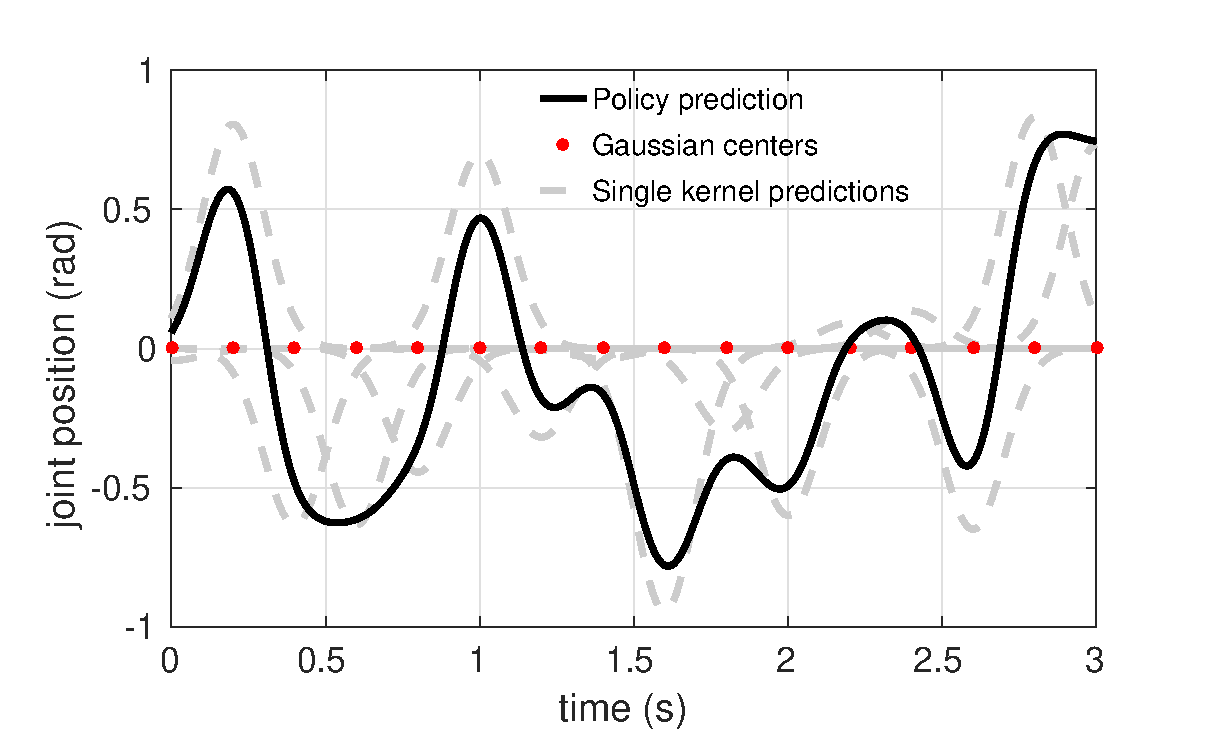
\includegraphics[scale=.4]{example_gr3.eps} 
 \caption{Example of a policy encoded as a weighted average of 
 Gaussian kernels: the means $\mu_i$ are equally spaced and the 
 variances are all fixed to $0.01$ and the weights have been 
 sampled from $[-1,1]$.}
 \vspace*{-5mm}
  \label{fig:policy_example}
\end{figure}


\section{Simulation Results}

We present the results obtained on a realistic simulation of the 
HyQ2Max robotic platform, as detailed in the previous section. All policies are 
encoded with a fixed set of $M=16$ Gaussian kernels evenly spaced in the time interval
between $0$ to $T$ seconds, while their variance $\sigma^2$ is fixed to $0.01$. 
The number of samples for each task is determined by the CMAS-ES algorithm,
based on the number of decision variables.

\subsection{Rearing}

In the rearing scenario, the quadrupedal system starts from a neutral, 
four legged support pose (Fig. \ref{fig:rearing_behaviour} (left)). 
During the task execution the front legs push the torso upwards, while the lower legs are 
supporting the body. This behavior can serve as a preliminary stage for much 
more complex maneuvers (e.g., obstacle traversing, transition to bipedal 
posture). We note that in general such postures cannot be reached in a static 
manner. To further reduce the complexity of the problem, we exploit the task 
structure and impose the same policy for the front and hind leg pairs,
respectively.

The policy is initialized to values that maintain the default pose of the system, 
in four legged support (Fig. \ref{fig:rearing_behaviour}, left).
The policy converged to a feasible solution within approximately 3002 trials
($177$ evaluation episodes with $17$ samples per episode), for an allocated time 
horizon of $T=0.3\;s$. The values of the weights used for this task were 
$Q_{1} = 10^3, \; Q_{2} = 10^2, \; Q_{3} = 0.1, \; Q_{4} = 1$.

\begin{figure}[h!]
 \centering
 \vspace*{+4mm}
 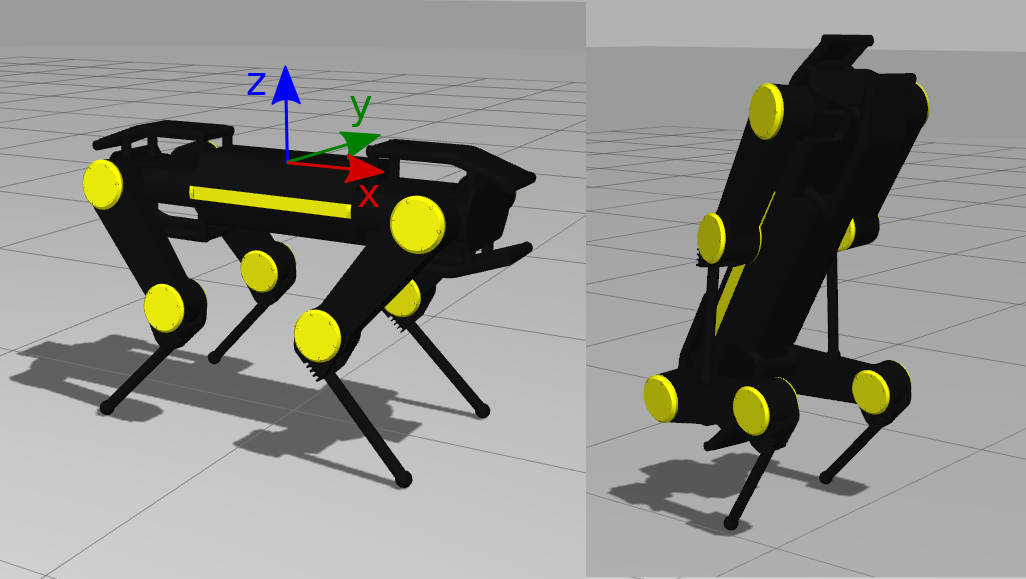
\includegraphics[scale=.25]{rearing_befor_after_ins.png} 
 \caption{HyQ2Max performing the rearing task in simulation under the resultant 
policy. \textit{Left:} initial pose.
 \textit{Right:} final pose.}
%   \vspace*{-3mm}
  \label{fig:rearing_behaviour}
\end{figure}

Fig. \ref{fig:rearing_behaviour} (right) shows the final pose reached by the 
system under the resultant policy, as imposed by the requirements on the 
position and orientation of the trunk, encoded in the terminal cost $p$. 
In the case of rearing we designated these only as the desired torso pitch ($-1.0472\; rad$)
and CoM (center of mass) height ($90\; cm$), leaving the other dimensions free for the optimization. 
The target pose was achieved with an accuracy of $0.006\; rad$  and $10 \; cm$, the performance is
reflecting the relative ratios of the cost function weights.

\begin{figure}[h!]
 \centering
 \hspace*{-8mm}
 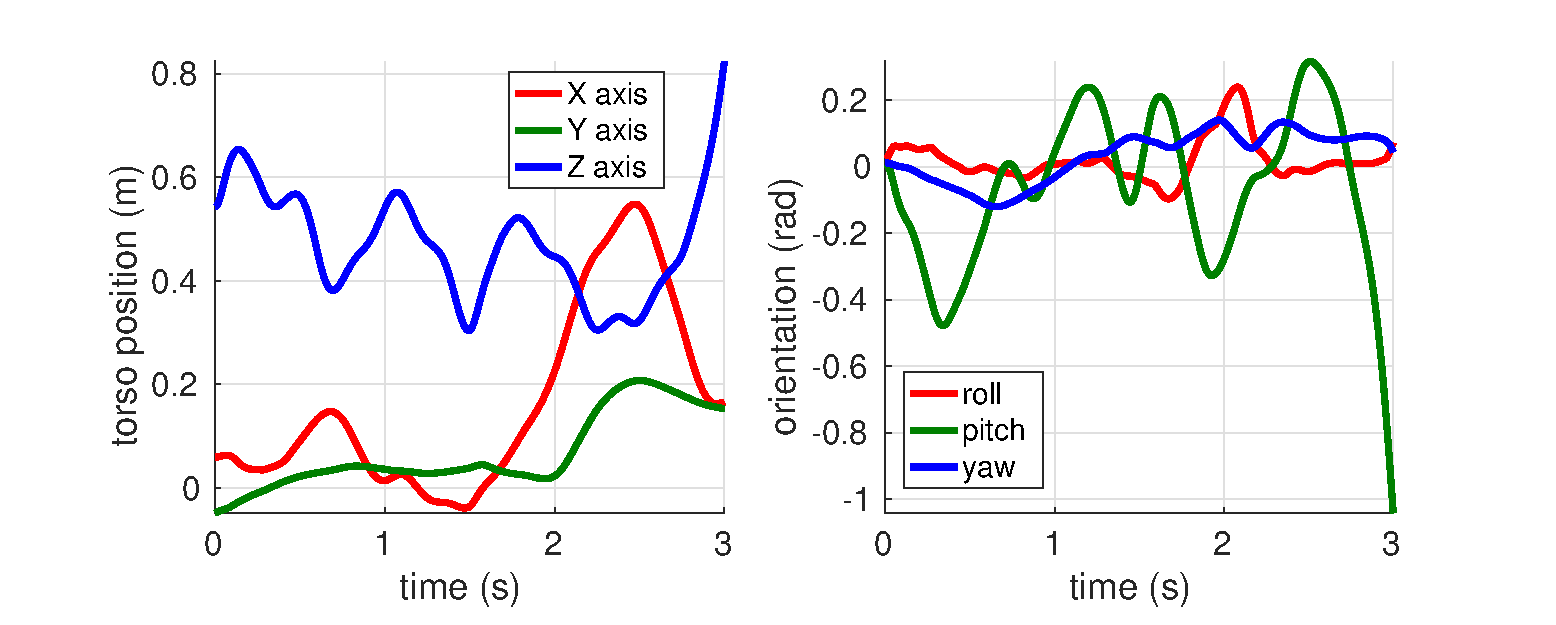
\includegraphics[scale=.37]{PRec_solution_joints_1_ICRA.eps} \\
 \small
  (a) Trunk trajectories (trunk CoM) of HyQ2Max performing the rearing task under the resultant policy. \\
  Body position (\textit{left}) and orientation (\textit{right}) in the world frame.
  \hspace*{-4mm}
  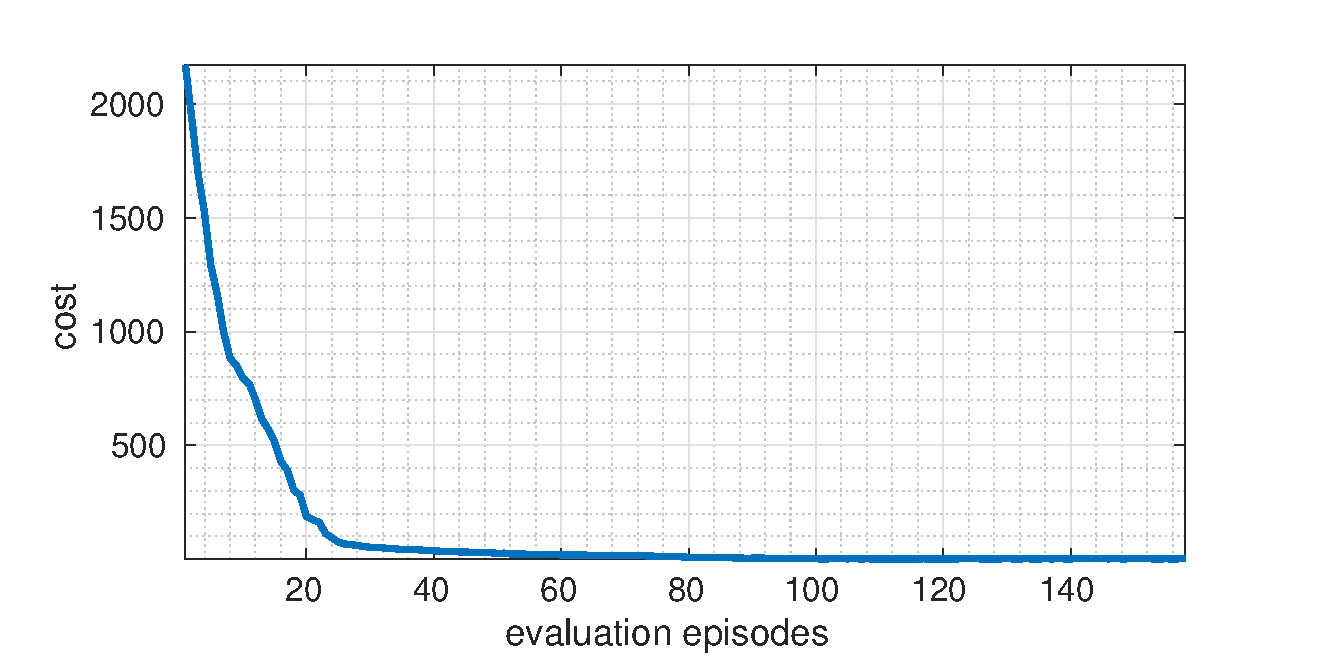
\includegraphics[scale=.37]{PRec_solution_1_ICRA.eps}\\
  (b) Evolution of the cost for the rearing experiment\\ ($158$ evaluation episodes with $19$ samples per episode)
  \normalsize
  \caption{ Joint trajectory solution for the HyQ2Max platform in the rearing task:
  (a) Resultant trunk trajectory. (b) Cost evolution.}
%    \vspace*{-3mm}
  \label{fig:rearing_plots}
\end{figure}

\begin{figure}[h!]
 \centering
 \vspace*{-3mm}
 \hspace*{-5mm}
%  \begin{subfigure}[b]{0.53\textwidth}
    \centering
  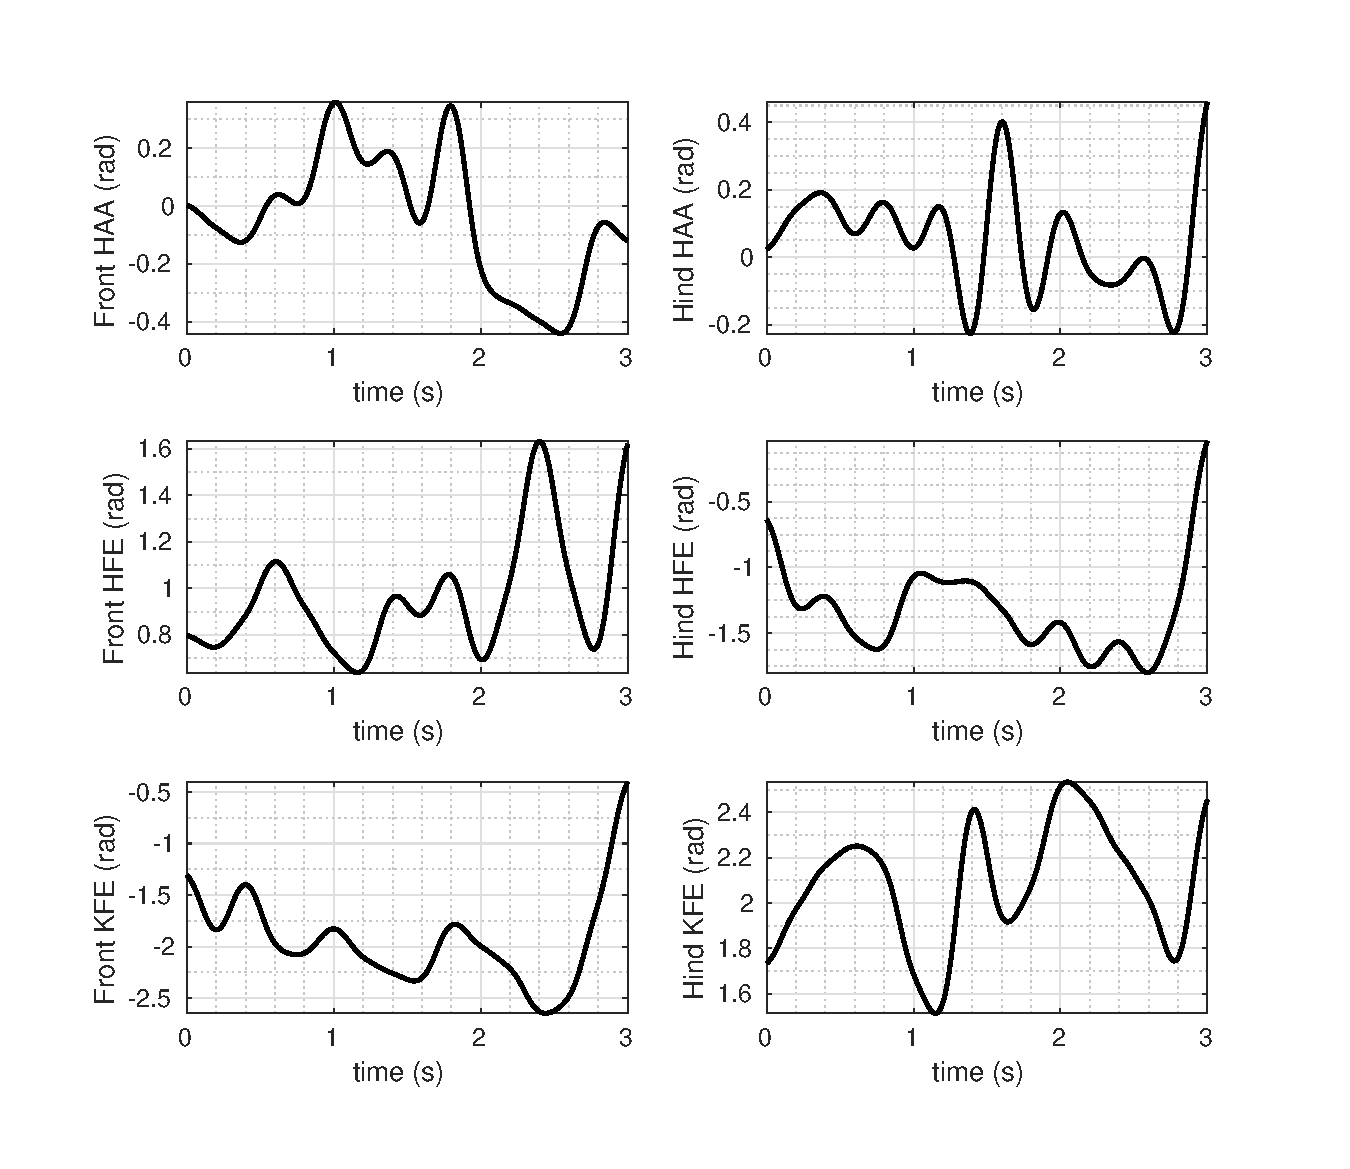
\includegraphics[width=0.53\textwidth]{rearing_GaussSol_1_ICRA_e.eps}
%  \end{subfigure}
%  \begin{subfigure}[b]{0.5\textwidth}
%    \vspace*{-4mm}
%    \hspace*{2mm}
%    \centering
%    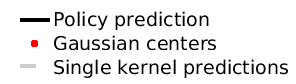
\includegraphics[width=0.4\textwidth]{Legend.png}
%  \end{subfigure}
 \caption{The optimized joint trajectories for the rearing task on the HyQ2Max 
platform. We impose the same policy for the front and hind leg pairs. 
Each limb has 3 actuators : HAA (hip abduction/adduction), HFE (hip flexion extension) and KFE (knee 
flexion/extension).}
   \vspace*{-4mm}
  \label{fig:rearing_gauss}
\end{figure}

The evolution of the position and orientation of the robot's trunk for the 
final trial are depicted in Fig. \ref{fig:rearing_plots}, alongside the evolution 
of the cost throughout the CMAS-ES (Fig. \ref{fig:rearing_plots}-(b)). 
The resultant individual joint policies (with the hind and front leg pairs sharing the
same policies) are displayed in Fig. \ref{fig:rearing_gauss}.

% The evolution of the position and orientation of the robot's trunk for the 
% final trial is depicted in Fig. \ref{fig:rearing_plots}, 
% with each individual policy taking a shape similar to that in Fig. 
% \ref{fig:policy_example} (a). The evolution of the cost throughout the CMAS-ES
% exploration is depicted in Fig. \ref{fig:rearing_plots} (b).

\subsection{Posture recovery}

For the task of posture recovery we introduce a scenario where the regular 
locomotion task fails, due to an unexpected obstacle, and the robot finds itself in an unforeseen,
fallen state (Fig. \ref{fig:sr_behaviour}, left). The task consists of returning the system to
an upright position, that allows the resuming of the locomotion task. Unlike in the rearing scenario, due to 
the nature of the task, the individual leg policies are independent of each other.

The final cost $p$ penalizes deviations from a target final state of the robot's 
trunk (in both linear and angular DoF). The values of the weights used for this task were 
$Q_{1} = 10^3, \; Q_{2} = 10^3, \; Q_{3} = 0.1, \; Q_{4} = 1$.
The desired final pose was defined as a neutral orientation ($\bq^{*}_{B} = (roll, \: pitch, \; yaw) = (0, 0, 0)$),
while the position was specified only by CoM (center of mass) height ($61\; cm$), leaving the other dimensions free for the optimization. 

The policy converged to a feasible solution within approximately 3002 trials 
($158$ evaluation episodes with $19$ samples per episode), 
with a time horizon $T=0.3\;s$. The desired pose was achieved with an accuracy 
of $0.001\; rad$  and $2 \; cm$. As in the previous scenario, the performance is
reflecting the relative ratios of the cost function weights.

Fig. \ref{fig:sr_behaviour} (middle) shows an intermediary pose reached 
by the system under the resultant policy. Fig. \ref{fig:sr_behaviour} 
(right) depicts the final pose after the policy is executed and the current 
goal is maintaining the pose. 
The trajectories of the position and orientation of the robot's trunk in the final
solution are depicted in Fig. \ref{fig:poseRec} (a).
The evolution of the cost function from initial plan to the delivered solution 
is depicted in Fig. \ref{fig:poseRec} (b). 
The resultant individual joint policies are displayed in Fig. \ref{fig:poserec_gauss}.

\begin{figure*}[t!]
 \centering
  \vspace*{+4mm}
 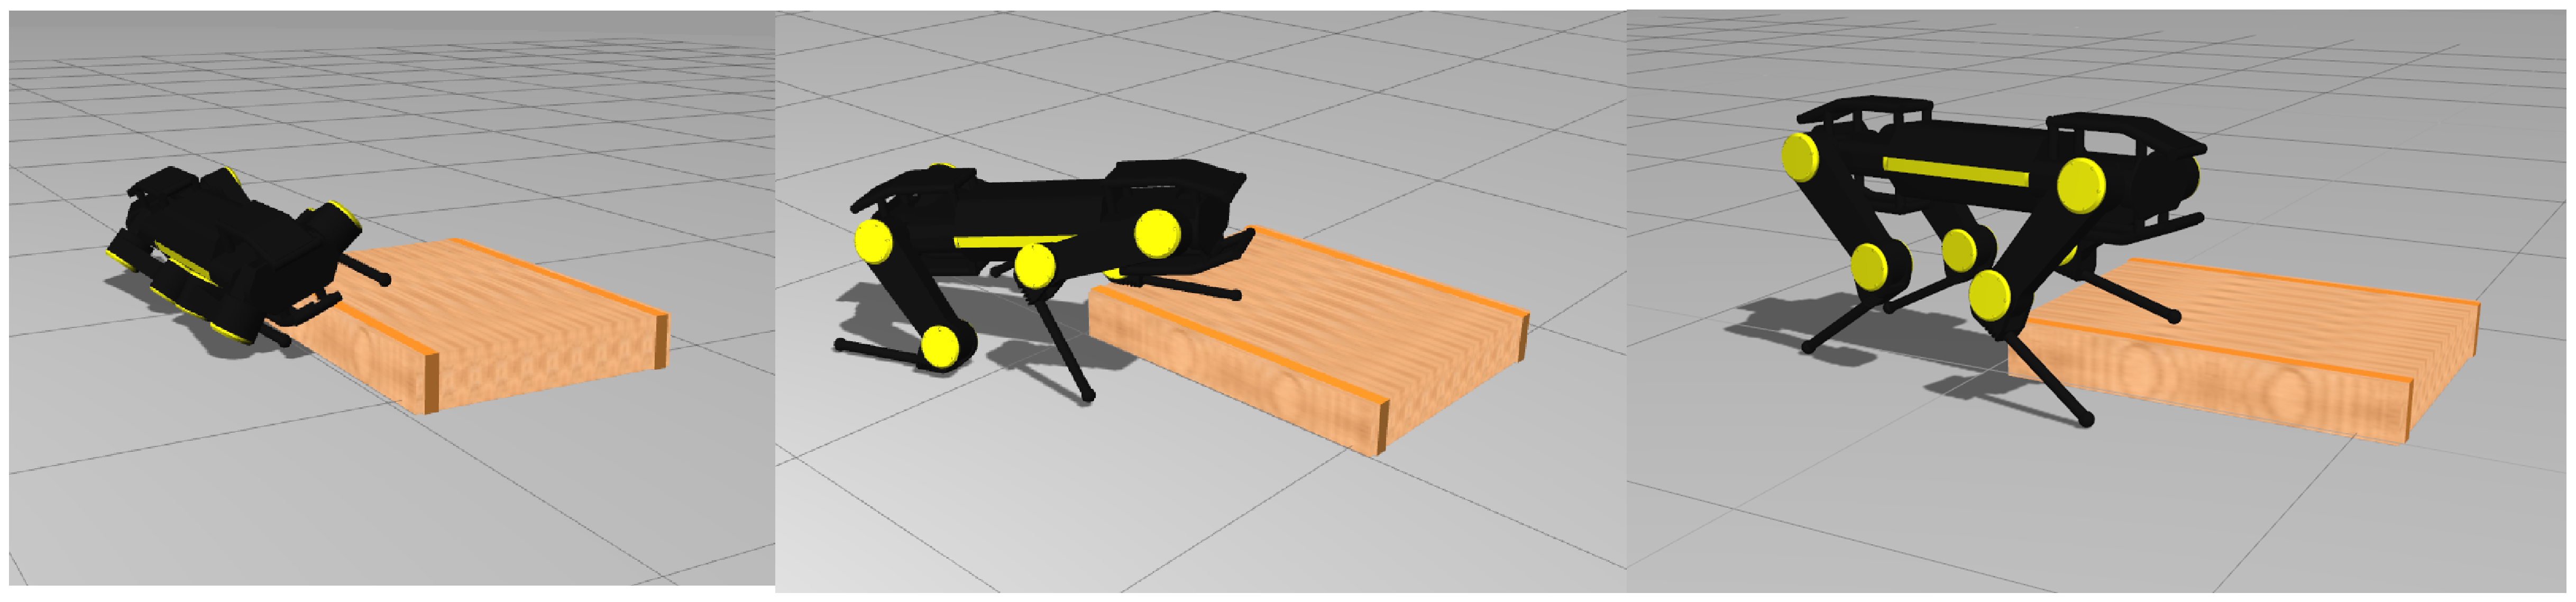
\includegraphics[scale=.2]{sr_befor_after_new.eps} 
 \caption{HyQ2Max performing the posture recovery task in simulation. 
\textit{Left:} initial pose (unexpected fall, ending up partially on an obstacle). 
\textit{Middle:} intermediary pose under the resultant policy.
 \textit{Right:} final pose (after the policy is executed and the current 
goal is maintaining the pose).}
   \vspace*{-4mm}
  \label{fig:sr_behaviour}
\end{figure*}

\begin{figure}[h!]
 \centering
 \hspace*{-7mm}
 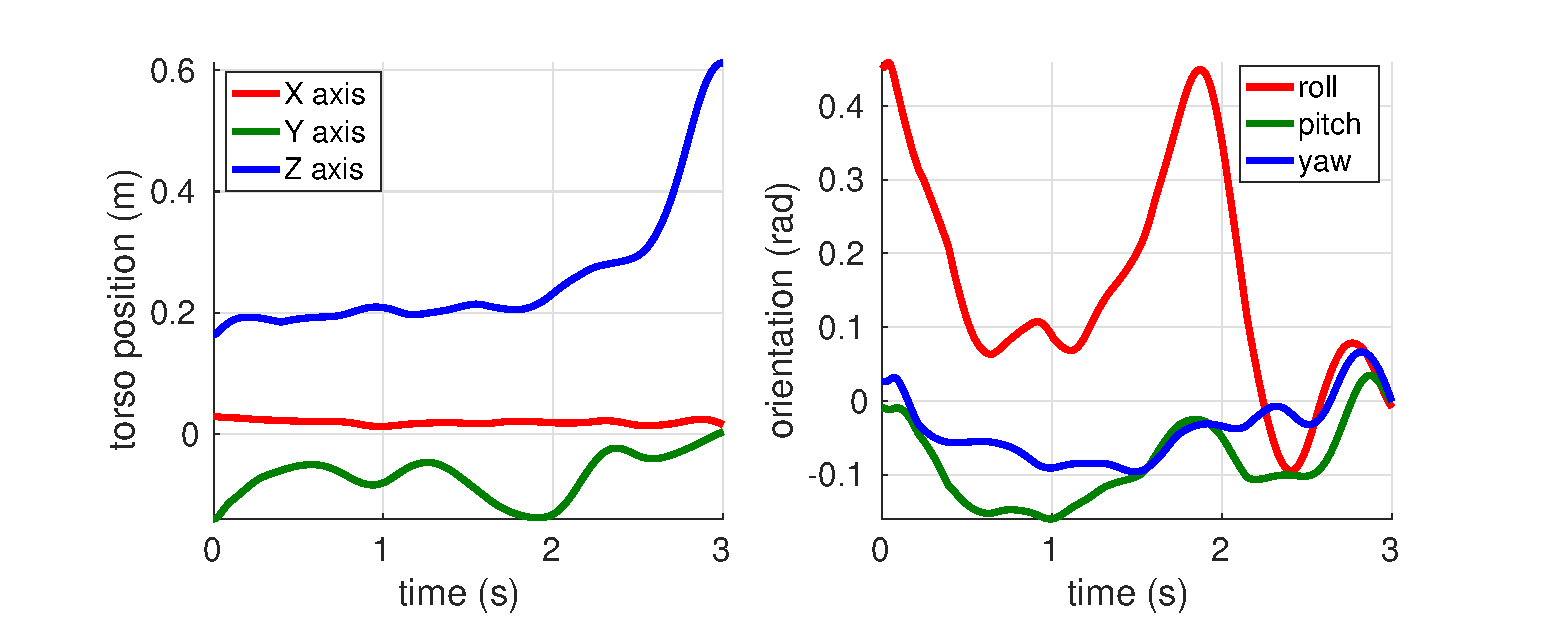
\includegraphics[scale=.37]{sr_solution_1_ICRA.eps} \\
 \small
  (a) Trunk trajectories (trunk CoM) of HyQ2Max performing the posture recovery task under the resultant policy. \\
  \textit{Left:} absolute body position.  \textit{Right:} body orientation.
  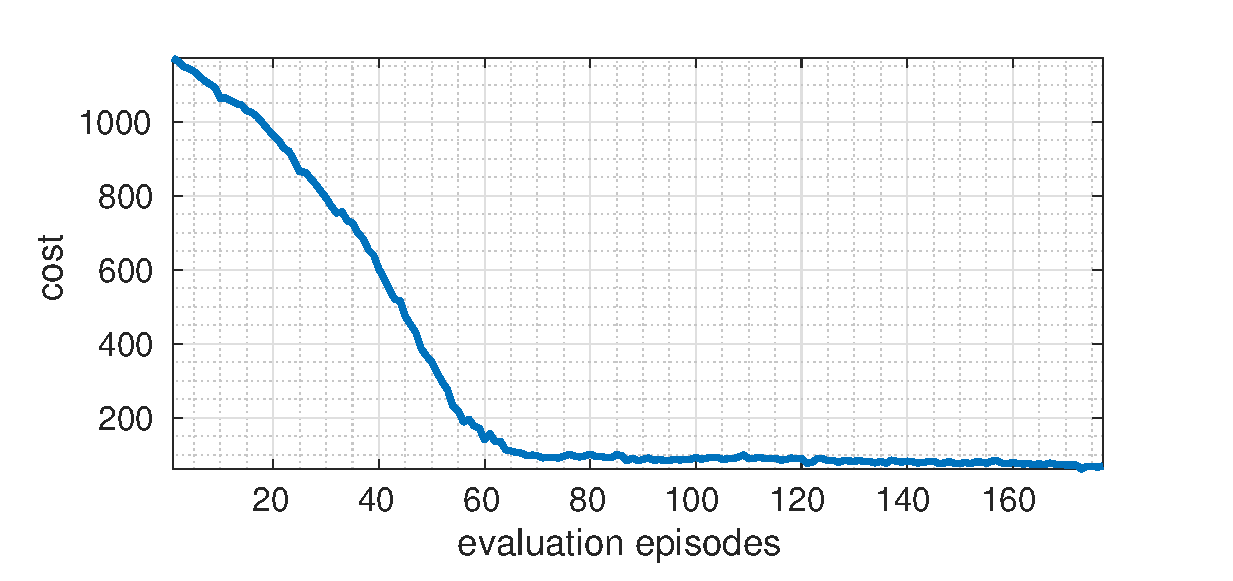
\includegraphics[scale=.45]{sr_cost_1_ICRA.eps}\\
  (b) Evolution of the cost for the posture recovery experiment\\ ($177$ evaluation episodes with $17$ samples per episode)
  \normalsize
  \caption{Joint trajectory solution for the HyQ2Max platform in the posture recovery task: 
  (a) Resultant trunk trajectory (position and orientation). (b) Cost evolution.}
     \vspace*{-4mm}
  \label{fig:poseRec}
\end{figure}

\begin{figure}[h!]
   \vspace*{-3mm}
    \begin{subfigure}[b]{0.52\textwidth}
        \centering
        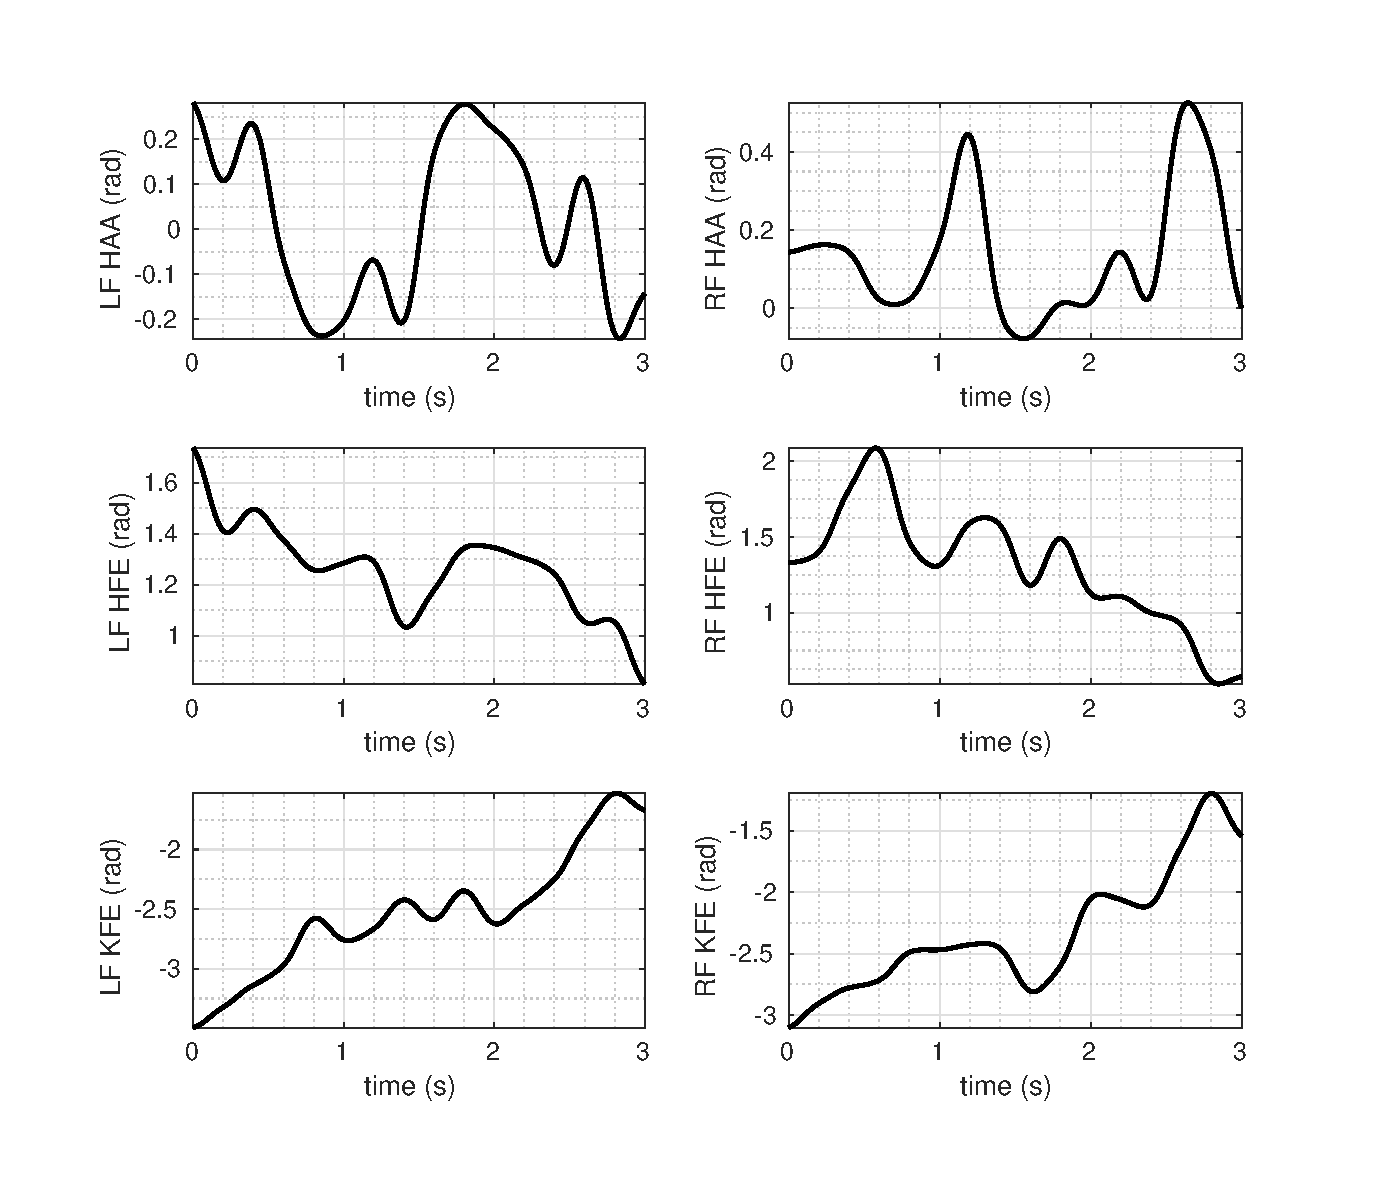
\includegraphics[width=\textwidth]{PRec_GaussSol_1of2_ICRA_e.eps}
    \end{subfigure}
    \begin{subfigure}[b]{0.52\textwidth}
     \vspace*{-5mm}
     \centering
     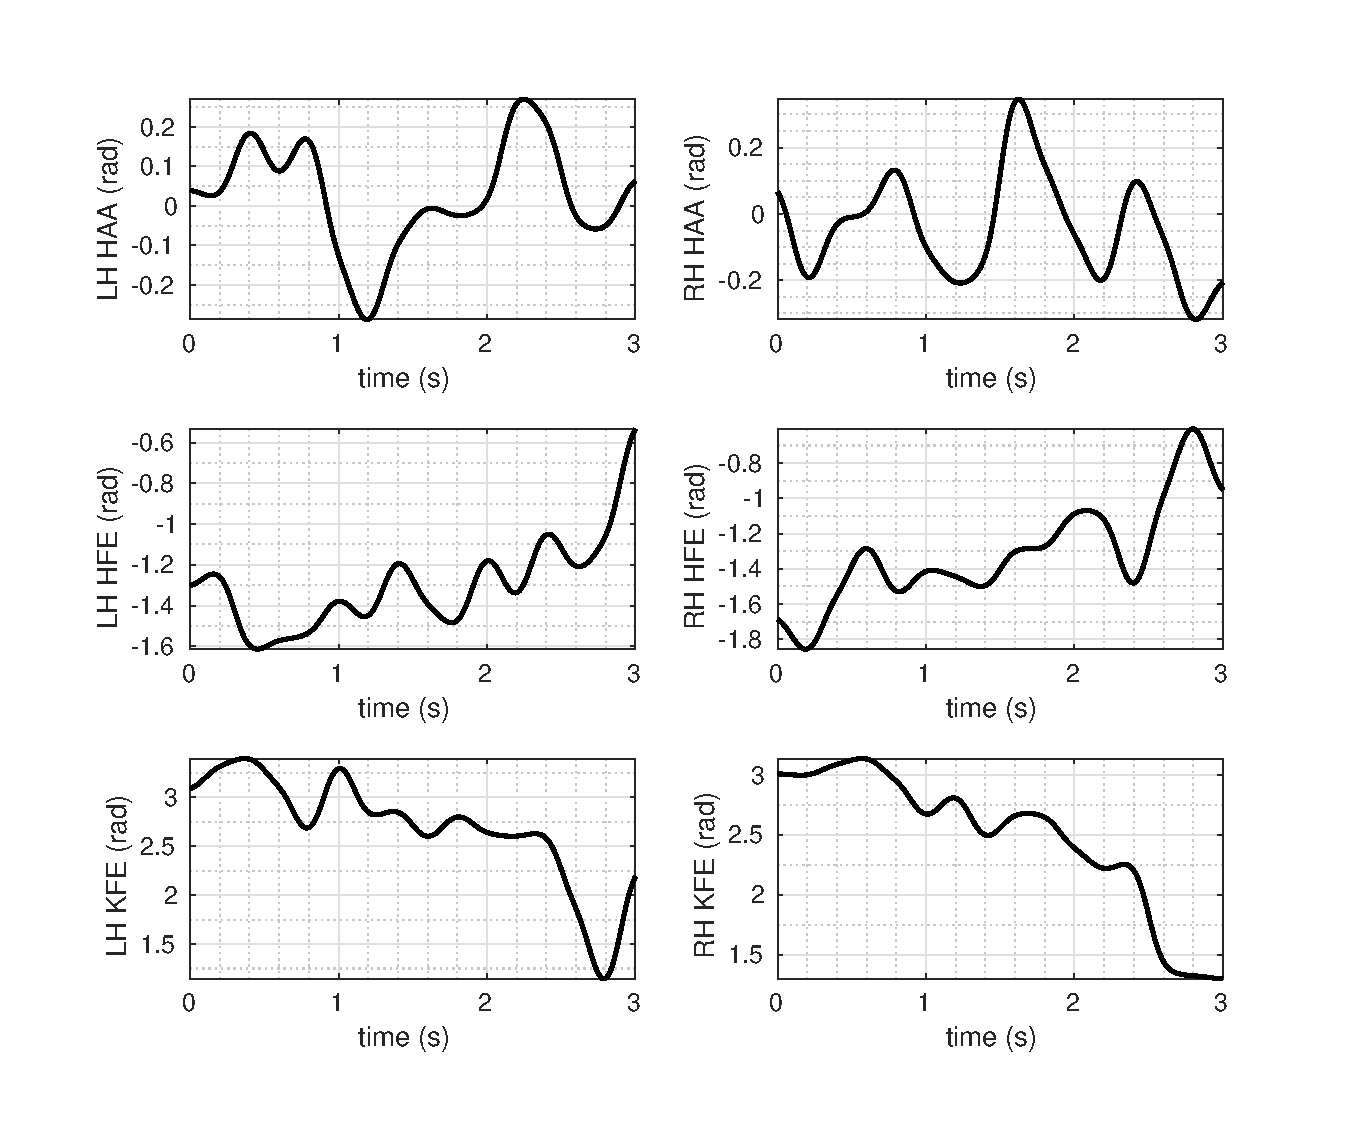
\includegraphics[width=\textwidth]{PRec_GaussSol_2of2_ICRA_e.eps}
%      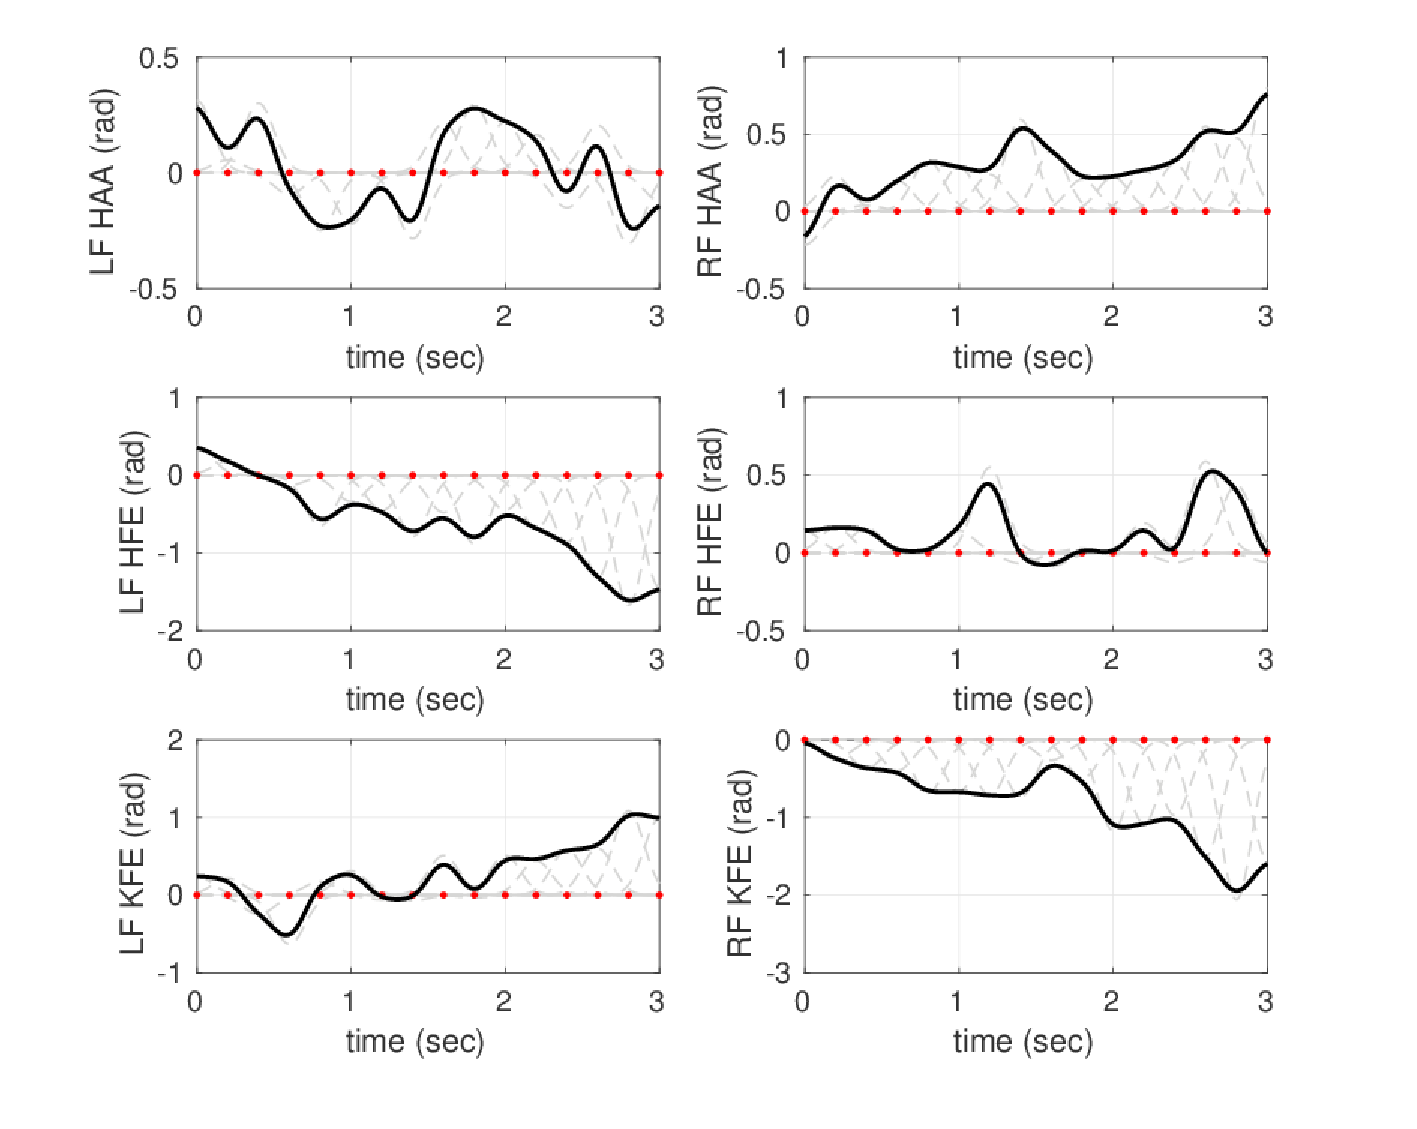
\includegraphics[width=\textwidth]{PRec_GaussSol_2of2_ICRA_e_trans.eps}
    \end{subfigure}
%     \begin{subfigure}[b]{0.5\textwidth}
%      \vspace*{-3mm}
%      \hspace*{2mm}
%      \centering
%      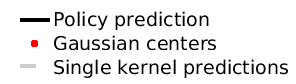
\includegraphics[width=0.4\textwidth]{Legend.png}
%     \end{subfigure}
    \caption{The optimized joint trajectories for the posture recovery task on the 
HyQ2Max platform. (LF - left front, RF - right front, LH - left hind, RH - 
right hind).}
   \vspace*{-5mm}
    \label{fig:poserec_gauss}
\end{figure}

% The simulation results indicate that the behaviour can be transferred to the real hardware.
The presented results suggest that the obtained behaviors could be transferred to
the real hardware, which is what we are focusing on implementing in the near future.
By enforcing high gains on the torque and joint limits' costs, the feasibility of
the whole body trajectory generated can be achieved. 
At the same time we are aiming to expand the range of posture recovery and extend the approach
to full body self-righting. A video of the presented results and behaviors is available in the
additional material or at the following link.\footnote{\url{https://youtu.be/irZTaTgwdoE}}

% The current results are limited to the simulation environment in the context
% of relatively simple scenarios. The presented results indicate that the behaviour 
% can be transferred to the real hardware, which we we aim to achieve in the near future, while
% expanding the range posture recovery and rearing scenarios addressed. 

% \section{Experiments}

\section{Conclusion}

In this work we present a whole body optimization methodology for non-periodic 
dynamic movements on quadrupedal systems. The approach is able to deliver 
trajectory solutions which involve multiple contacts, without any predefined
feet placement heuristics (e.g., contact points, timing or order of succession). 

Using a realistic simulation of the hydraulically actuated HyQ2Max quadrupedal system 
we investigate two distinctive tasks: rearing and posture recovery. Task specific
cost functions encode the high-level goals in each scenario. We employ a
generalized form for the cost function, while adjusting the relative gains of each term 
according to the current task. Although tuning the relative weights of such cost functions is a manual 
process, a heuristic encoding of the same behavior would require a significantly higher effort.
By exploiting the whole body model in order to obtain the solution, the optimization does not have
to depend upon heuristics and can overcome errors caused by the use of simplified models.
The resultant trajectories and the accuracy with which the user defined goals are achieved are 
reflecting the relative ratios of the weights on the individual cost function terms. 

\section{Future directions}

The results depicted in this work showcase the possibilities that optimization 
can offer to motion synthesis for complex, non-periodic tasks. For example, the goal of a rearing 
motion can be to reach the basin of attraction of a balancing controller, 
keeping the quadruped upright. In future work we aim to transfer the obtained 
behaviors onto the hardware system, while also expanding the 
range of scenarios addressed.

As the future task of the system was beyond the scope of this investigation, certain elements,
(e.g., the allocated time and final velocities of the trunk) were not included in the
optimization goals. We aim to extend the approach to deliver an
optimal duration for the given task, while the final pose is fully determined, based on
subsequent requirements. To increase the autonomy of the system under the suggested approach, real-time 
sensory information from the environment and a methodology for determining 
the ideal final pose of the policy will have to be integrated. 
In the long term we aim to develop a general tool for generating optimal dynamic 
whole-body motions that are not necessarily periodic in nature.

The speed of computing such solutions might not always allow for on-line
optimization using conventional approaches. Machine learning methods (in conjunction with an adequate motion library)
could be employed to speed up the solution delivery time. 
In \cite{mordatch2014combining} the solutions of an optimization task are 
used to guide the learning of neural network controllers, for a variety of 
locomotion tasks on generic robotic models in simulation. Such dynamic 
movements will serve in complementing and extending the capabilities of robots 
with arms and legs.

% \section*{Acknowledgement}
% 
% This research is funded by the Fondazione Istituto Italiano di Tecnologia.
% The authors would like to thank the following people for their support and
% assistance for the success of this project: Roy Featherstone, Marco Frigerio,
% Victor Barasuol, Michele Focchi, Carlos Mastalli, Marco Camurri, Bilal Ur Rehman, 
% Romeo Orsolino, Alex Posatskiy, Yifu Gao, Felipe Polido, Jose Colmenares, 
% and our team of technicians.
% \renewcommand{\baselinestretch}{0.9}

\bibliographystyle{IEEEtran}
% \bibliographystyle{ieeetr}
\bibliography{icra17radulescu}

\end{document}
